\documentclass{report}

\usepackage{ugentstyle}

\usepackage{listings}

\begin{document}
	\maketitle{Besturingssystemen III}

	\tableofcontents

	\chapter{WMI concepten}
	\section{Herhaling SNMP en inleiding WMI}
	SNMP had de mogelijkheid om informatie bij te houden van devices die typisch op een netwerk aangesloten zijn zoals printers, routers, workstations en servers. Er was echter nood aan een systeem dat ook informatie van het hele operating systeem kon bevragen.
	Dit systeem noemt \textit{Wbem}, een uniform systeem voor het bevragen van besturingssystemen zoals windows, HP en solaris. Een Windows specifieke versie hiervan is het \textit{Windows Management Instrumentation} (WMI). Uit figuur \ref{fig:basisarchitectuur_WMI} kunnen vijf componenten afgeleid worden:
	\begin{figure}[h]
		\centering
		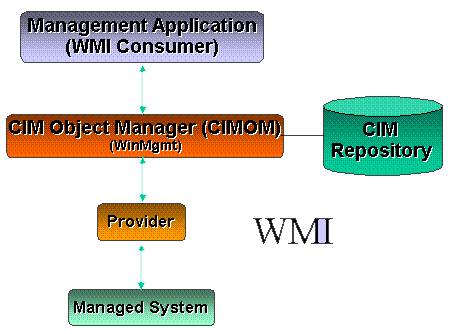
\includegraphics[width=0.5\textwidth]{basisarchitectuur_WMI}
		\caption{Basisarchitectuur WMI}
		\label{fig:basisarchitectuur_WMI}
	\end{figure}


	\begin{itemize}
		\item \textit{WMI Consumer} : Dit zijn gebruikersapplicaties die gebruik maken van de CIMOM (= de WMI Service) om diverse informatie op te vragen. Deze kunnen in diverse programmeertalen geprogrammeerd worden (in dit vak wordt Perl gebruikt).
		\item \textit{CIM Object Manager} : Wordt ook de WMI Service genoemd en heeft drie functionaliteiten: 
		\begin{enumerate}
			\item Interactie met de WMI Consumer op een \textbf{uniforme} manier.
			\item De WMI Service is verantwoordelijk voor alle communicatie met de pr oviders. De WMI Consumer hoeft niets te weten over de verzameling Providers. De WMI Service gebruikt de CIM Repository om de juiste Provider te raadplegen.
			\item De CIM Repository is enkel toegankelijk voor de WMI Service
		\end{enumerate}
		\item \textit{CIM Repository}. Dit is een databank zowel waarbij software als hardware componenten als objecten voorgesteld worden.  Deze object georiënteerde methode zorgt ervoor dat deze componenten via methoden kunnen aangesproken worden. Voor elke klasse wordt ook bijgehouden door welke provider deze klasse gerealiseerd wordt.
		\item \textit{Provider} : Een provider is verantwoordelijk voor een aantal WMI-klassen
		\item \textit{Managed System} : Dit zijn hardware componenten die aangesloten zijn aan een werkstation.
	\end{itemize}
	\section{CIM Repository}
	De CIM Repository kan men inspecteren met een WMI-browser. Voorbeelden hiervan zijn \textit{WMI CIM Studio} en \textit{Powershell WMI Browser}. In deze samenvatting wordt gebruik gemaakt van WMI CIM Studio
	De inlogprocedure vraagt een namespace die standaard ingevuld staat op \texttt{root:\\CIMV2}. Deze namespace omvat ook de meeste WMI Objecten. Wat deze namespace niet heeft zijn klassen om office documenten zoals excel of word te manipuleren.
	Indien ingelogd, verschijnt er een scherm met twee panelen. Het linkerpaneel bevat alle klassen gesorteerd op hiërarchische volgorde op basis van overerving. De icoontjes naast elke klasse wordt gegenereerd op basis van de attributen van die klasse.
	Het rechterpaneel heeft standaard de \textit{Properties} tab open. Dit tabblad bevat alle attributen van de geselecteerde klasse. Attributen voorafgegaan door 2 underscores zijn systeemattributen en bestaan voor elke klasse.
	Voorbeelden van zulke systeemattributen:
	\begin{itemize}
		\item \_\_DERIVATION : Dit bevat een tabel met de hiërarchie van de overerving waarbij het eerste element de onmiddelijke superklasse is en het laatste element de root van de hiërarchie.
		\item \_\_DYNASTY : Dit bevat de root van de hiërarchie van overerving. Deze informatie is dus dezelfde als het laatste element in het \_\_DERIVATION attribuut.
		\item \_\_PROPERTY\_COUNT : Dit veld bevat een nummer met het aantal niet-systeemaanroepen
		\item \_\_PATH : Dit veld bevat het absolute pad van de klasse.
	\end{itemize}
	Van elke klasse kan zijn instanties opgevraagd worden door op het icoontje rechts van het save-icoontje te klikken. Er wordt een twee dimensionale tabel weergegeven met per instantie een rij en per attribuut een kolom.
	Voor elke instantie moet het systeemattribuut \_\_RELPATH aangevuld worden met de sleutel van het object. Dit is een string dat bestaat uit meerdere key-value paren dat toegevoegd wordt aan de default waarde van \_\_RELPATH.
	Bij Singletons echter zijn unieke identificaties niet nodig en wordt \_\_RELPATH aangevuld met een \@ symbool. Een voorbeeld van een abstracte klasse en een singleton is respectievelijk \texttt{CIM\_MonitorResolution} en \texttt{Win\_LocalTime}. 
	\section{Qualifiers}
	Een qualifier is een key-value koppel waarbij extra eigenschappen kunnen toegevoegd worden. Er bestaan vier soorten qualifiers:
	\begin{enumerate}
		\item klasse-qualifiers. Geeft extra informatie over de klasse. 
		\item attribuut-qualifiers. Geeft extra informatie over de attributen van een klasse
		\item methode-qualifiers. Geeft extra informatie over de methoden van een klasse
		\item methodeparameter-qualifiers. Geeft extra informatie over de parameters van de methoden van een klasse.
	\end{enumerate}
	\subsubsection{Klasse-qualifiers}
	Deze worden in WMI CIM Studio \textit{Object qualifiers} genoemd:
	\begin{itemize}
		\item De \textbf{Description} qualifier geeft tekst terug met informatie over de klasse.
		\item De \textbf{Abstract}, \textbf{Dynamic} en \textbf{Singleton} qualifiers geven aan, indien hun waarde op \textit{true} staat, dat een klasse abstract, dynamisch of een singleton is.
		\item De \textbf{Provider} qualifier helpt de WMI service te bepalen welke provider moet aangesproken worden om een bepaalde klasse aan te spreken
	\end{itemize}
	\subsubsection{Attribuut-qualifiers}
	De attribuut-qualifiers worden in WMI CIM Studio \textit{Property qualifiers} genoemd:
	\begin{itemize}
		\item De \textbf{Description} qualifier geef analoog zoals de klasse-qualifiers tekst terug met informatie over het attribuut.
		\item De \textbf{CIMType} qualifier geeft het type van het attribuut weer, zoals string, boolean, datetime, signed of unsigned int (8, 16, 32 of 64 bits) of referenties naar absolute objectpaden.
		\item De \textbf{Write} qualifier geeft aan, indien deze op \textit{true} staat, dat de het attribuut rechtstreeks wijzigbaar is, zonder hiervoor methodes te moeten aanspreken. 
		\item De \textbf{Keys} qualifier geeft aan dat het attribuut deel uitmaakt van de sleutel van het object en bijgevolg ook vermeld moet worden in het objectpad van een instantie.
		\item ValueMap geeft in een ééndimensionale tabel het domein weer van het attribuut: een expliciete opsomming van de toegelaten waarden.
			  Values geeft een meer informatieve interpretatie van de toegelaten waarden. Indien ook de ValueMap qualifier aanwezig is, kunnen ValueMap en Values best beschouwd worden als respectievelijk de keys en de values van een Perl hash. Indien een ValueMap ontbreekt, dan impliceert Values een ValueMap met oplopende gehele getallen, startend vanaf 0. Values kan dan geïnterpreteerd worden als een Perl array.
	\end{itemize}
	\subsubsection{Methode-qualifiers}
	\begin{itemize}
		\item De \textbf{Description} qualifier geeft uitleg over de methode.
		\item De \textbf{CIMType} qualifier specifieert het return type.
		\item De \textbf{ValueMap} en \textbf{Values} worden vaak gebruikt bij een integer returnwaarde om deze waarde te vertalen naar iets zinvols.
		\item De \textbf{Privileges} qualifier specifieert een lijst van privileges die nodig zijn om de methode op te roepen. Indien deze qualifier niet aanwezig is kan eender wie de methode uit voeren.
	\end{itemize}
	De bijzonderste methode is de \textit{Create} methode. Dit is een statische methode die onafhankelijk is van een specifieke instantie. 
	
	Een voorbeeld van een klasse met enkel statische methoden is \textbf{StdRegProv}. Deze klasse bevat methoden die het register kan aanpassen. 
	
	\subsubsection{Methodeparameter-qualifiers}
		\begin{itemize}
			\item De Description, CIMType, Values en ValueMap qualifiers hebben een analoge functie als de corresponderende attribuut- en methodequalifiers, nu toegepast op een individuele parameter van een methode.
			\item \textbf{In/Out} geeft aan dat deze parameter een invoer- (resp. uitvoer-) parameter is. Een parameter kan ook invoer/uitvoer parameter zijn.
			\item De \textbf{Optional} qualifier, indien ingevuld op true, geeft aan dat deze parameter optioneel is. Voor elke optionele qualifier is er wel een default waarde.
			\item \textbf{ID} geeft de volgorde aan (startend met de waarde 0) waarin de parameters als argumenten bij de methodeaanroep moeten opgegeven worden.
		\end{itemize}
	
	\section{Associatorklassen}
	Stel dat je informatie wenst over de ethernet adapter. De klasse \textbf{Win32\_NetworkAdapter} klasse kan allesinds de ethernet adapter filteren, maar er ontbreekt informatie zoals het IP adress. Die informatie bevindt zich in een andere klasse, \textbf{Win32\_NetworkAdapterConfiguration}. In beide klasse zijn er echter geen verwijzingen naar de andere klasse. Voor zowel 1:1, 1:n en m:n relaties gebruikt WMI associatorklassen. Dit zijn klassen met meestal 2 attributen die een klasse met een andere klasse associeert. Eén van de instanties van de associatorklasse \textbf{Win32\_NetworkAdapterSetting} zal in het eerste attribuut \textit{element} een verwijzingen hebben naar de ethernet adapter in Win32\_NetworkAdapter en zal in het tweede attribuut \textit{setting} een verwijzing hebben naar de ethernet adapter in Win32\_Network-AdapterConfiguration zodat deze informatie gecombineerd kan worden.
	
	\section{WMI Query Language}
	WMI Consumers kunnen gebruik maken van \textbf{WQL}, een querytaal gebaseerd op SQL waarbij enkel de \texttt{SELECT}, \texttt{FROM} en \texttt{WHERE} clausule beschikbaar zijn. Clausules zoals \texttt{GROUP BY}, \texttt{HAVING} en \texttt{JOIN} zijn \textit{niet} mogelijk in WQL. Het opvragen van alle ethernetadapters wordt bereikt met volgend stukje WQL code:
	\begin{lstlisting}
select * 
from win32_networkadapter
where netconnectionid = 'Ethernet'
	\end{lstlisting}
	Attributen die gebruikt worden zijn niet hoofdlettergevoelig. Query's kunnen uitgetest worden in het programma \textbf{wbemtest.exe}. Bij het opstarten moet er eerst geconnecteerd worden naar een namespace dat standaard ingevuld is op \textit{root\textbackslash cimv2}. Indien op de knop \textit{Query} geklikt wordt zal er een venster verschijnen waarin WQL queries kunnen uitgevoerd worden. Het is ook mogelijk om de instanties op te vragen die gelinkt zijn aan het doelobject via associatorklassen.
	
	
	\begin{lstlisting}
associators of {win32_directory.name="C://..."}
where resultclass=win32_directory
resultrole=partcomponent
	\end{lstlisting}
	Verschillende predicaten in de \textit{where} clausule worden niet verbonden met het AND keywoord zoals men verwacht, deze wordt namelijk impliciet ingevuld.
	\section{Notification queries}
	Een WMI Consumer kan zich aanmelden aan de WMI Service indien deze een interesse heeft voor een bepaalde gebeurtenis. De provider weet welke consumers geïnteresseerd en zal dan ook de consumers inlichten wanneer de voorwaarden voldaan zijn. Een consumer hoeft hier zelf geen processortijd aan te spenderen. Bij het uittesten van notification queries staat de optie \textit{asynchronous} best in \textit{Wbemtest} aan, anders is de uitvoeringstijd langer. Een voorbeeld van een notification query:
	\begin{lstlisting}
select * 
from win32_processtrace
where processname = "calc.exe"
	\end{lstlisting}
	Deze query zal de consumer inlichten wanneer een windows rekenmachine opgestart of afgesloten wordt met een \textbf{Win32\_ProcessTrace} object. In een notification query kan ook geaggregeerd worden. Deze komt zo goed als overeen als de SQL group by clausule, behalve dat er nog een extra sleutelwoord komt: \texttt{WITHIN}. Een \texttt{WITHIN} extensie specifieert het interval in seconden wanneer er geaggregeerd moet worden. Er is verder ook nog een \texttt{HAVING} clausule, die exact dezelfde functie heeft als bij SQL. Volgend voorbeeld zal om de 5 seconden enkel geaggregeerde informatie tonen indien meer dan 5 processen van het type \textit{calc.exe} of \textit{notepad.exe} aangemaakt of gesloten worden. Eerst wordt er geaggregeerd op de processnaam, daarna wordt er nog onderscheidt gemaakt tussen het type klasse. Dit is ofwel \textbf{Win32\_ProcessStartTrace} of \textbf{Win32\_ProcessStopTrace}.
	\begin{lstlisting}
select * 
from win32_processtrace
where (processname = "calc.exe"
    or processname = "notepad.exe)
group within 5 by processname, __CLASS
having numberofevents >= 5
	\end{lstlisting}
	
	De geaggregeerde informatie komt in een object \_\_AggregateEvent. Zo een object heeft slechts twee attributen:
	\begin{enumerate}
		\item \textit{NumberOfEvents}: Dit geeft aan hoeveel events er zijn afgevuurd binnen het interval van de within extensie.
		\item \textit{Representative}: Dit attribuut verwijst naar één van deze gebeurtenissen. Informatie over de andere events gaan verloren.
	\end{enumerate}

	Een spijtige zaak is dat notification queries maar voor een beperkt aantal providers mogelijk is. Indien eventobjecten voor een bepaald object niet bestaan moet men beroep doen op het \textbf{snapshotmechanisme}. In de query komt er een \texttt{WITHIN} extensie, die functioneel verschillend is van de \texttt{WITHIN} extensie van de group by. Deze nieuwe \texttt{WITHIN} extensie zal een interval in seconden aangeven waarop een nieuwe snapshot moet gemaakt worden. Verder is er nog de \texttt{ISA} operator. Deze operator laat toe om een variabele met een klasse te vergelijken.
	
	Volgend voorbeeld illustreert dezelfde query, zonder de group by clausule en met behulp van de \textbf{\_\_InstanceOperationEvent} klasse, om events te genereren bij het aanmaken of vernietigen van processen met de naam calc.exe en notepad.exe.
	\begin{lstlisting}
select *
from __instanceoperationevent 
within 2
where (__CLASS = "__instancecreationevent"
    or __CLASS = "__instancedeletionevent")
and targetinstance isa 'win_32_process'
and (targetinstance.name = "calc.exe" 
  or targetinstance.name = "notepad.exe")

	\end{lstlisting}
	
	Een belangrijke klasse is de \textbf{\_\_TimerEvent} klasse. Deze eventklasse wordt gegenereerd door de klasse \textbf{\_\_TimerInstruction}, die twee implementaties kent: \textbf{\_\_AbsoluteTimerInstruction} en \textbf{\_\_IntervalTimerInstruction}. Dit zijn ook direct twee van de weinige klassen waarvan je zelf instanties mag van maken. De klasse \textbf{\_\_AbsoluteTimerInstruction} is niet zo interessant aangezien die maar één enkele event zal afvuren op een specifiek tijdstip. De \textbf{\_\_IntervalTimerInstruction} klasse daarentegen, zal een event afvuren telkens het interval bereikt wordt. De klasse bevat twee belangrijke attributen: \textit{TimerID}, een unieke identificatie van de timer en \textit{IntervalBetweenEvents}, het interval in milliseconden tussen opeenvolgende events. Vanaf dat een instantie van een \textbf{\_\_IntervalTimerInstruction} gemaakt wordt, kan via volgende notification query dit event onderschept worden
	\begin{lstlisting}
select *
from __timerevent
where timerid=...
	\end{lstlisting}
	waarbij ... vervangen wordt door het gewenste \textit{TimerID}. In het slechtste geval kan dit ook dienen als pollingsmechanisme, als snapshots ook niet werken.
	
	\section{Consumerprogrammas}
	Windows voorziet een aantal consumerprogrammas. Twee interessante zijn \textbf{SMTPEventConsumer} en \textbf{CommandLineEventConsumer}.
	\subsection{SMTPEventConsumer}
	Zoals de naam het doet vermoeden, zal deze consumer een mail sturen bij het afvuren van een specifiek event. Ten eerste moet er een instantie gemaakt worden van de klasse \textbf{\_\_EVENTFILTER}. Belangrijke attributen zijn: \textit{QueryLanguage}, dat best ingesteld wordt op WQL, \textit{query}, een WQL query en \textit{name}, een unieke identificatie. Nu kan een instantie gemaakt worden vand e klasse \textbf{SMTPEventConsumer}. Deze klasse heeft de volgende belangrijke attributen:
	\begin{itemize}
		\item \textit{Name}: een unieke identificatie.
		\item \textit{ToLine}: het e-mailadres van de ontvanger.
		\item \textit{FromLine}: het e-mailadres van de vertegenwoordiger van de mail.
		\item \textit{Subject}: het onderwerp van de mail.
		\item \textit{Message}: het bericht van de mail.
		\item \textit{SMTPServer}: een smtpserver, bv die van Google.
	\end{itemize}

	Deze twee klassen moeten nog aan elkaar gelinkt worden. Dit wordt gerealiseerd met behulp van de associatorklasse \textbf{\_\_FilterToConsumerBinding}. Het attribuut \textit{Filter} moet het \_\_PATH attribuut bevatten van de gewenste filterinstantie. Het attribuut \textit{Consumer} moet het \_\_PATH attribuut bevatten van de gewenste consumerinstantie.
	
	Stel dat toegepast moet worden met volgende query:
	\begin{lstlisting}
select * 
from win32_processtrace
where (processname = "calc.exe"
or processname = "notepad.exe)
group within 5 by processname, __CLASS
having numberofevents >= 5
	\end{lstlisting}
	Het \textit{query} attribuut van de \textbf{\_\_EventFilter} klasse moet ingevuld worden met deze query. 
	De attributen van \textbf{SMTPEventConsumer} kunnen als volgt ingevuld worden:
	\begin{lstlisting}
Name=mail1
ToLine=bert.desaffel@gmail.com
FromLine=bert.desaffel@gmail.com
Subject=%Representative.__CLASS% %NumberOfEvents%
Message=%Representative.Name%
SMTPServer=smtp.ugent.be
	\end{lstlisting}
	
	\subsection{CommandLineEventConsumer}
	Deze consumer zal een command line commando uitvoeren na het afvuren van een specifiek event. De configuratie gebeurd op dezelfde manier als bij een \textbf{SMTPEventConsumer} instantie. Volgend voorbeeld gebruikt een \textbf{\_\_EVENTFILTER} instantie waarbij de query als volgt ingesteld is:
	\begin{lstlisting}
select *
from win32_processstarttrace
where processname = 'calc.exe'
	\end{lstlisting}
	De \textbf{CommandLineEventConsumer} wordt als volg geïnstantieert. Dit zal het proces dat net opgestart wordt, terug killen.
	\begin{lstlisting}
Name=command1
CommandLineTemplate=taskkill /f /pid %ProcessID%
	\end{lstlisting}

\end{document}


